\begin{frame}
    \frametitle{Functional Programming}
    \begin{block}{Why?}
        See Jeffrey's chalk talk
    \end{block}
    \begin{block}{Concepts}
        \begin{columns}
            \begin{column}{0.5\textwidth}
                \begin{itemize}
                    \item No state change
                    \item No side effects
                    \item Function composition is crucial
                    \item What about IO?
                \end{itemize}
            \end{column}
            \begin{column}{0.5\textwidth}
                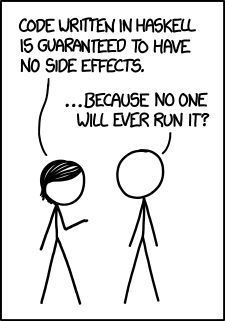
\includegraphics[scale=0.5]{images/xkcd}
            \end{column}
        \end{columns}
    \end{block}
\end{frame}
\begin{frame}
    \frametitle{Demystification}
    \begin{block}{}
        \begin{itemize}
            \item A monad is not a specific feature.
            \item They are simple data structures that happen to implement the monadic interface
            \item Being a monad is simply adhering to a certain(monadic) interface (bind, unit)
        \end{itemize}
    \end{block}
\end{frame}
\begin{frame}
    \frametitle{Monads}
    \begin{block}{Disclaimer}
        No guarantees.
    \end{block}
\end{frame}
